%%%%%%%%%%%%%%%%%%%%%%%%%%%%%%%%%%%%%%%%%%%%%%%%%%%%%%%%%%%%%%%
%
% Edit your LaTeX on the left, and it gets compiled for you on 
% the right. If you give someone the link to this page, they 
% can edit at the same time. See the help menu above for more 
% info. Enjoy!
%
%%%%%%%%%%%%%%%%%%%%%%%%%%%%%%%%%%%%%%%%%%%%%%%%%%%%%%%%%%%%%%%
\documentclass[11pt]{article}
\usepackage{fancyhdr}
\usepackage{graphicx}
\usepackage{amssymb}
\usepackage{epstopdf}
\usepackage{amsmath} 	
\usepackage{amssymb}
\usepackage{cite}
\usepackage{multirow}
\usepackage{wrapfig}
\usepackage{subfigure}
\usepackage{todonotes}
\usepackage{listings}
\usepackage{float}
\usepackage[colorlinks=true, linkcolor=black,citecolor=black,urlcolor=blue]{hyperref}
\bibliographystyle{IEEEtran}
\DeclareGraphicsRule{.tif}{png}{.png}{`convert #1 `dirname #1`/`basename #1 .tif`.png}

%---------------- Letter Paper --------------------%
% be sure to change in document class too
\textwidth = 6.5 in
\textheight = 8.6 in
\oddsidemargin = 0.0 in
\evensidemargin = 0.0 in
\topmargin = 0.0 in
\headheight = 0.0 in
\headsep = 0.2in
\parskip = 0.2in
\parindent = 0.0in

\newcommand{\keyword}[1]{\textit{#1}}

\begin{document}
\thispagestyle{empty}
\begin{center}
\vspace*{1.5in}
{\LARGE \textbf{PROJECT TITLE}} %<---- Insert your project title here

{\Large MCHE 201: Introduction to Mechanical Design\\ \vspace*{0.1in} Spring 2015}

\vspace*{2.5in}

% author names and CLIDS
\begin{figure}[!h]
\begin{minipage}{0.45\textwidth}
\begin{center}
Author 1 \\
Department of Mechanical Engineering\\
University of Louisiana at Lafayette\\
Lafayette, LA 70504\\
{\tt CLID1@louisiana.edu}
\end{center}
\end{minipage}
\hspace{0.08\textwidth}
\begin{minipage}{0.45\textwidth}
\begin{center}
Author 2 \\
Department of Mechanical Engineering\\
University of Louisiana at Lafayette\\
Lafayette, LA 70504\\
\tt{CLID2@louisiana.edu}
\end{center}
\end{minipage}
\end{figure}
%
\vspace{0.2in}
\begin{figure}[!h]
\begin{minipage}{0.45\textwidth}
\begin{center}
Author 3 \\
Department of Mechanical Engineering\\
University of Louisiana at Lafayette\\
Lafayette, LA 70504\\
{\tt CLID3@louisiana.edu}
\end{center}
\end{minipage}
\hspace{0.08\textwidth}
\begin{minipage}{0.45\textwidth}
\begin{center}
Author 4 \\
Department of Mechanical Engineering\\
University of Louisiana at Lafayette\\
Lafayette, LA 70504\\
\tt{CLID4@louisiana.edu}
\end{center}
\end{minipage}
\end{figure}

\end{center}

\newpage
\thispagestyle{empty}
\begin{abstract}
\vspace{-0.2in}
Aliquam aliquet, est a ullamcorper condimentum, tellus nulla fringilla elit, a iaculis nulla turpis sed wisi. Fusce volutpat. Etiam sodales ante id nunc. Proin ornare dignissim lacus. Nunc porttitor nunc a sem. Sed sollicitudin velit eu magna. Aliquam erat volutpat. Vivamus ornare est non wisi. Proin vel quam. Vivamus egestas. Nunc tempor diam vehicula mauris. Nullam sapien eros, facilisis vel, eleifend non, auctor dapibus, pede. Ut nulla. Vivamus bibendum, nulla ut congue fringilla, lorem ipsum ultricies risus, ut rutrum velit tortor vel purus. In hac habitasse platea dictumst. Duis fermentum, metus sed congue gravida, arcu dui ornare urna, ut imperdiet enim odio dignissim ipsum. Nulla facilisi.
\end{abstract} 

\newpage
\setcounter{page}{1} % reset the page counter, so it begins with the page of the introduction section
%%%%%%%%%%%%%%%%%%%%%%%%%%%%%%%%%%%%%%%%%%%%%%%%%%%%%%%%%%%%%%%%
%%%%%%%%%%%%%%%%%%%%%%%%%%%%%%%%%%%%%%%%%%%%%%%%%%%%%%%%%%%%%%%%
\section{Introduction}\label{sec:intro}

\vspace{-0.2in}
%
This is the introduction section\ldots Aliquam aliquet, est a ullamcorper condimentum, tellus nulla fringilla elit, a iaculis nulla turpis sed wisi. Fusce volutpat. Etiam sodales ante id nunc. Proin ornare dignissim lacus. Nunc porttitor nunc a sem. Sed sollicitudin velit eu magna. Aliquam erat volutpat. Vivamus ornare est non wisi. Proin vel quam. Vivamus egestas. Nunc tempor diam vehicula mauris. Nullam sapien eros, facilisis vel, eleifend non, auctor dapibus, pede. Ut nulla. Vivamus bibendum, nulla ut congue fringilla, lorem ipsum ultricies risus, ut rutrum velit tortor vel purus. In hac habitasse platea dictumst. Duis fermentum, metus sed congue gravida, arcu dui ornare urna, ut imperdiet enim odio dignissim ipsum. Nulla facilisi. 

Aliquam aliquet, est a ullamcorper condimentum, tellus nulla fringilla elit, a iaculis nulla turpis sed wisi. Fusce volutpat. Etiam sodales ante id nunc. Proin ornare dignissim lacus. Nunc porttitor nunc a sem. Sed sollicitudin velit eu magna. Aliquam erat volutpat. Vivamus ornare est non wisi. Proin vel quam. Vivamus egestas. Nunc tempor diam vehicula mauris. Nullam sapien eros, facilisis vel, eleifend non, auctor dapibus, pede. Ut nulla. Vivamus bibendum, nulla ut congue fringilla, lorem ipsum ultricies risus, ut rutrum velit tortor vel purus. In hac habitasse platea dictumst. Duis fermentum, metus sed congue gravida, arcu dui ornare urna, ut imperdiet enim odio dignissim ipsum. Nulla facilisi. 

%%%%%%%%%%%%%%%%%%%%%%%%%%%%%%%%%%%%%%%%%%%%%%%%%%%%%%%%%%%%%%%%
\section{Background}

%%%%%%%%%%%%%%%%%%%%%%%%%%%%%%%%%%%%%%%%%%%%%%%%%%%%%%%%%%%%%%%%
\section{Methods}\label{sec:methods}


\subsection{Solving the risk sensitive POMDP}
Marecki \cite{marecki} showed that RSPOMDPs can be solved for arbitrary utility functions using \keyword{reverse value iteration} in Belief Wealth Space.
For this the original state space must be augmented two times:

\begin{figure}[H]
\begin {center}
\begin {tikzpicture}[-latex ,auto ,node distance =3cm and 3cm ,on grid,
semithick , state/.style ={ circle ,fill=black!20, maximum width =2 cm}]
\node[state] (A) [align=center] {Observation\\Time\\Space};
\node[state] (B) [right of=A,align=center] {Belief\\Time\\Space};
\node[state] (C) [right of=B,align=center] {Belief\\Wealth\\Space};

\path (A) edge [line width=1mm, align=center] node[left] {} (B);
\path (B) edge [line width=1mm,align=center] node[below =0.25 cm] {} (C);
\end{tikzpicture}
\end{center}
\end{figure}

First augmentation is done by describing the probability of being in the good state with a function $\phi(b,o)$ ~\autoref{m:belief-update}:

\begin{align}
    b' = \phi(b,o) := ()
\end{align}

This augmentation transforms the POMDP into a MDP.
Second augmentation ...

%%%%%%%%%%%%%%%%%%%%%%%%%%%%%%%%%%%%%%%%%%%%%%%%%%%%%%%%%%%%%%%%

\section{Results}\label{sec:results}
\subsection{Solving the risk sensitive POMDP}

\normalsize
Marecki \cite{marecki} showed that RSPOMDPs can be solved for arbitrary utility functions using \textbf{reverse value iteration} in Belief Wealth Space.
For this the original state space must be augmented two times:

\begin{figure}
\begin {center}
\begin {tikzpicture}[-latex ,auto ,node distance =4cm and 2cm ,on grid,
semithick , state/.style ={ circle ,fill=black!20, minimum width =3 cm}]
\node[state] (A) [align=center] {Observation\\Time\\Space};
\node[state] (B) [right of=A,align=center] {Belief\\Time\\Space};
\node[state] (C) [right of=B,align=center] {Belief\\Wealth\\Space};


\path (A) edge [line width=2mm, align=center] node[left] {} (B);
\path (B) edge [line width=2mm,align=center] node[below =0.25 cm] {} (C);
\end{tikzpicture}
\end{center}
\end{figure}

\hspace{2cm}

\subsection{Value functions in belief wealth space}


\normalsize

\begin{figure}
    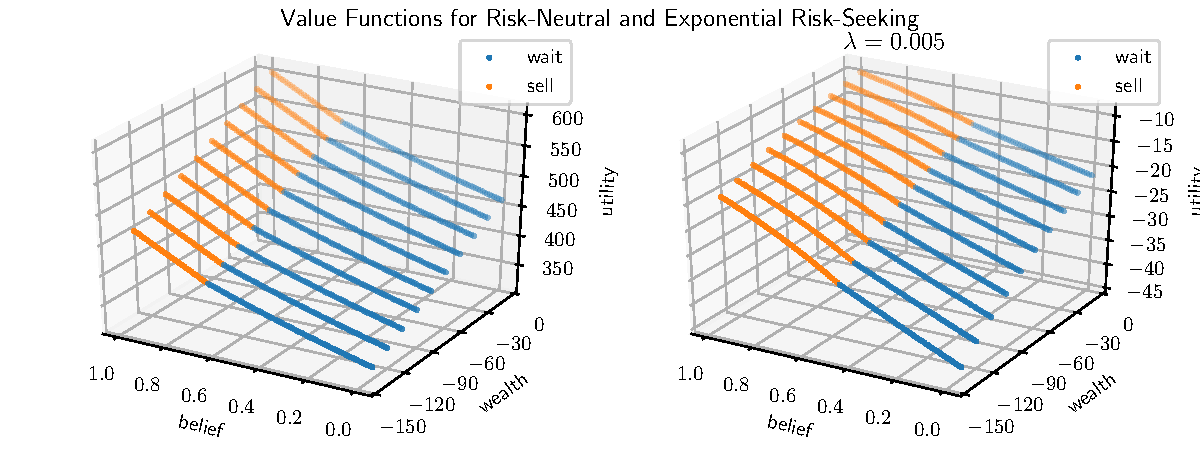
\includegraphics[width=0.98\linewidth]{img/exp_policy.pdf}\\
    \vspace{1cm}
    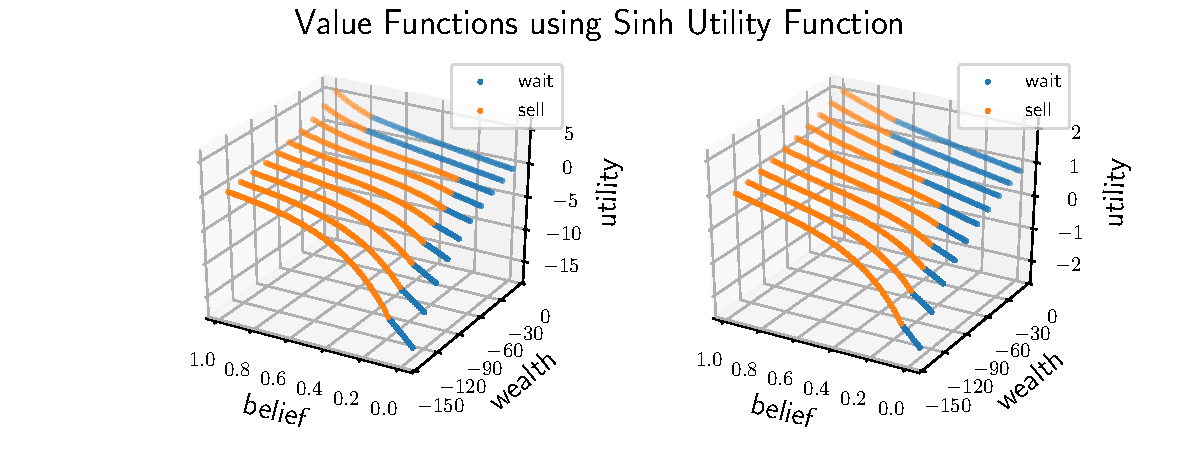
\includegraphics[width=0.98\linewidth]{img/sinh_policy.pdf}\\
    \vspace{1cm}
    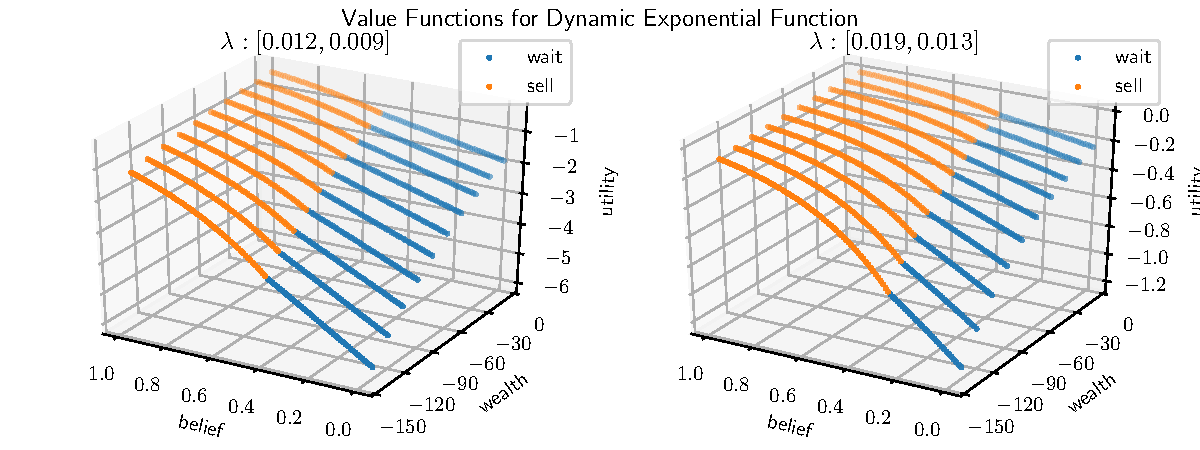
\includegraphics[width=0.98\linewidth]{img/dyn_policy.pdf}
    \caption{Value functions exhibiting different risk-behaviors; from top left: risk neutral agent (utility function is the identity function), risk-seeking agent with exponential utility function, two fixed time agents with different time thresholds, two agents with dynamic exponential utility function.}
\end{figure}

\subsection{From human behavior to utility functions}


\normalsize
\textbf{The original problem:}
\begin{itemize}
\item[①] Choose utility function with risk parameter.
\item[②] Perform value iteration.
\item[③] Derive policy.
\end{itemize}

\textbf{The inverse problem:}
\begin{itemize}
\item[①] Observe behavior.
\item[②] Estimate policy.
\item[③] Derive utility function and risk parameters.
\end{itemize}

The original problem is easy to solve, unfortunately for the inverse problem no solution is known. 

$\rightarrow$ Perform grid-search and choose optimal utility function.

\begin{figure}
    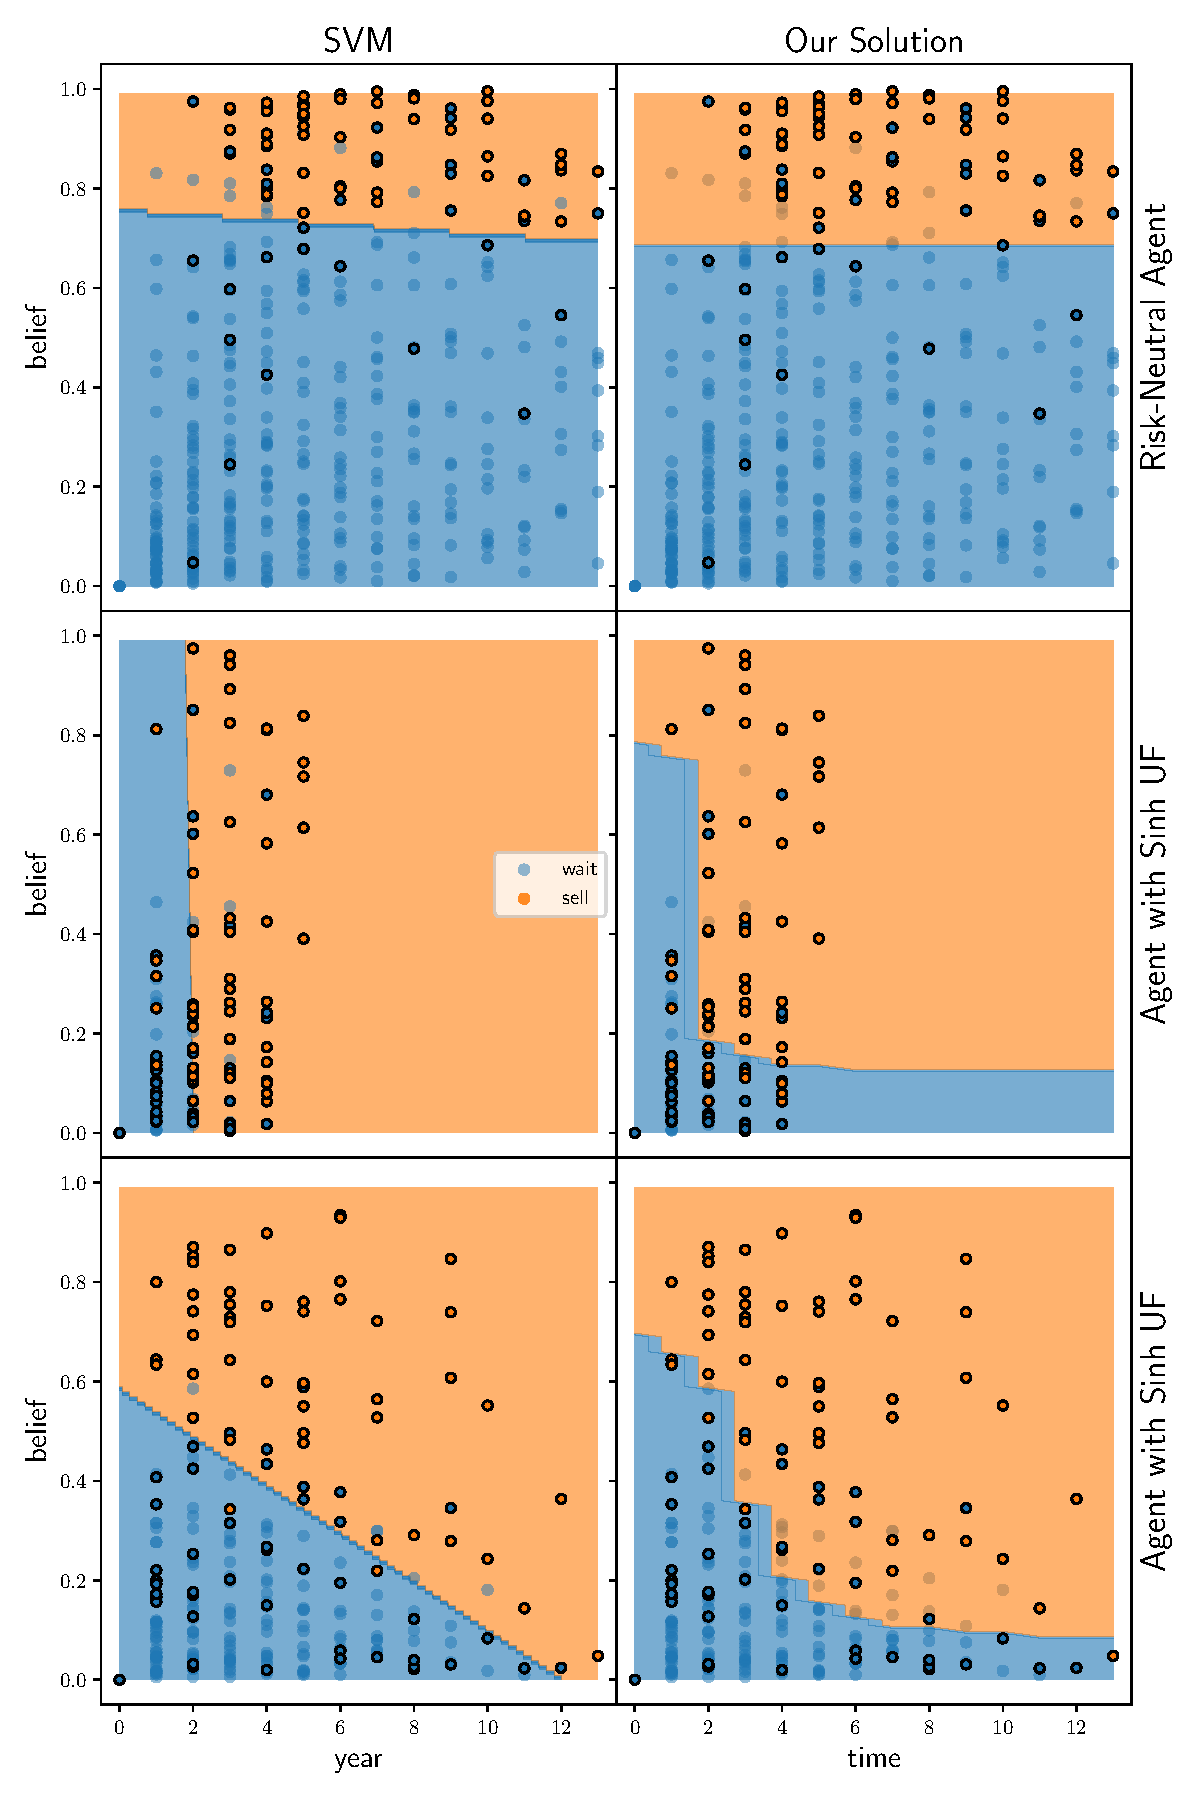
\includegraphics[width=0.8\linewidth]{img/fit}
    \caption{Examples from three human behaviors distinctly observed and replicated with RL agents. Behaviours by row: 1) Constant belief threshold, modelled by exponential utility, 2) Fixed time threshold, modelled by sinh utility, 3) Mixed strategy, modelled by dynamic exponential utility. Left column shows empirical optimal split of data using cross validation and linear kernel support vector machines, right column shows optimal policy found via gridsearch.}
    \label{fig:svm_vs_value}
\end{figure}

% TODO 6 boxes with only expensive expert and 3 behavior clusters.

\begin{figure}
% 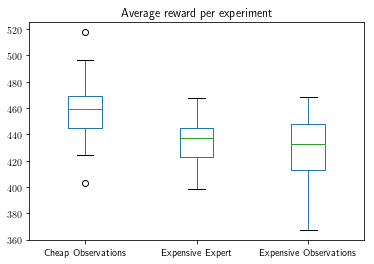
\includegraphics[width=0.4\linewidth]{img/avg_reward.png}
% 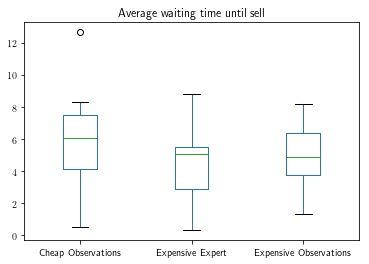
\includegraphics[width=0.4\linewidth]{img/avg_waiting.png}
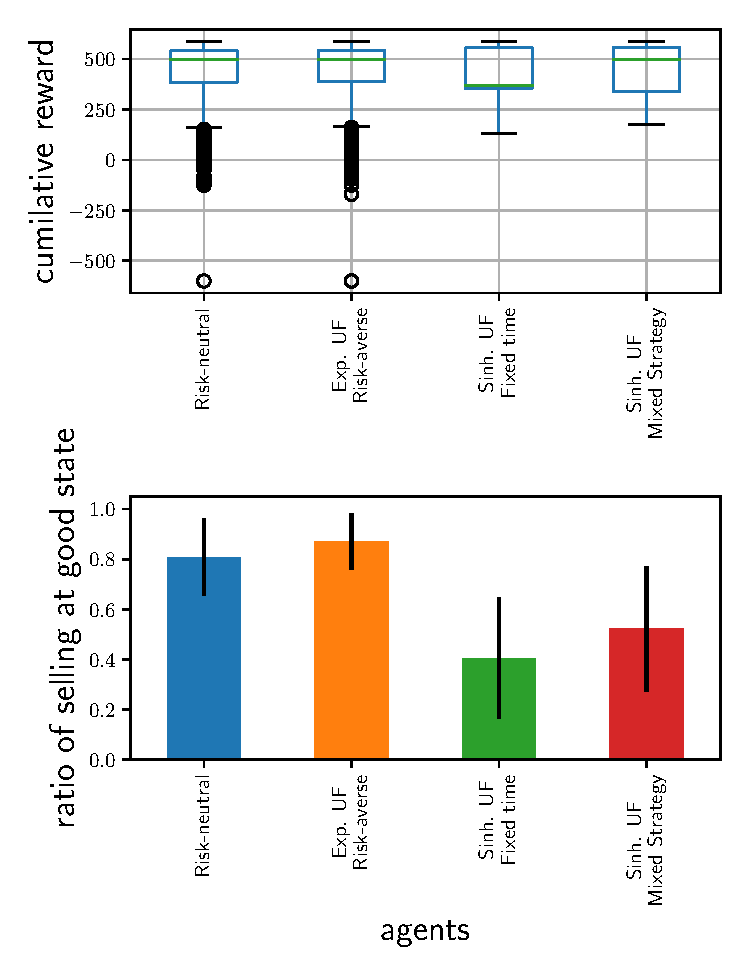
\includegraphics[width=0.8\linewidth]{img/performance.pdf}
\caption{Average reward and ratio of selling in the good state.}
\end{figure}



%%%%%%%%%%%%%%%%%%%%%%%%%%%%%%%%%%%%%%%%%%%%%%%%%%%%%%%%%%%%%%%%
\section{Conclusion}
\label{sec:conclusion}
\vspace{-0.2in}
%
Aliquam aliquet, est a ullamcorper condimentum, tellus nulla fringilla elit, a iaculis nulla turpis sed wisi. Fusce volutpat. Etiam sodales ante id nunc. Proin ornare dignissim lacus. Nunc porttitor nunc a sem. Sed sollicitudin velit eu magna. Aliquam erat volutpat. Vivamus ornare est non wisi. Proin vel quam. Vivamus egestas. Nunc tempor diam vehicula mauris. Nunc tempor diam vehicula mauris. Nullam sapien eros, facilisis vel, eleifend non, auctor dapibus, pede. Ut nulla. Vivamus bibendum, nulla ut congue fringilla, lorem ipsum ultricies risus, ut rutrum velit tortor vel purus.

\end{document}